\subsection{Example Videos}
\parbox{0.75\textwidth}{Every example in the book has an accompanying video; to view the video, click on the title of the example or the example number in the margin.}
\begin{center}
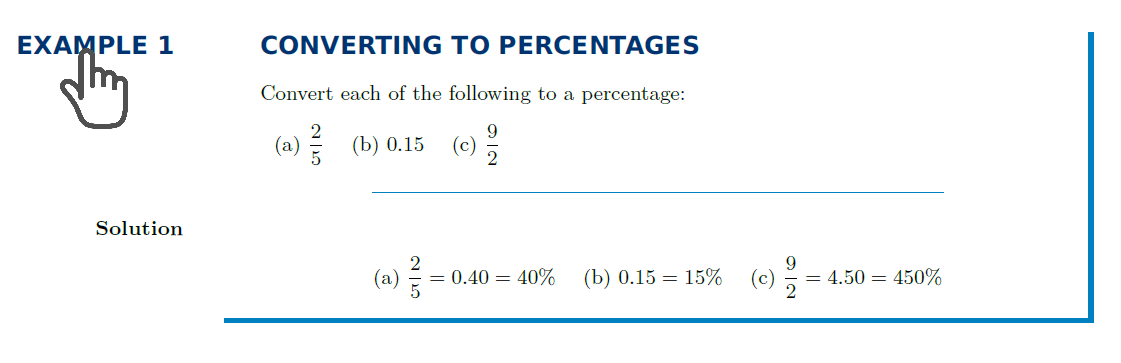
\includegraphics[width=0.75\textwidth]{examplehowto}
\end{center}

\subsection{Try It}
\parbox{0.75\textwidth}{Many examples are followed by Try It examples, which can be used for extra practice.  Clicking on the words Try It in the margin will open a web page where students can enter their answers and check them.}
\begin{center}
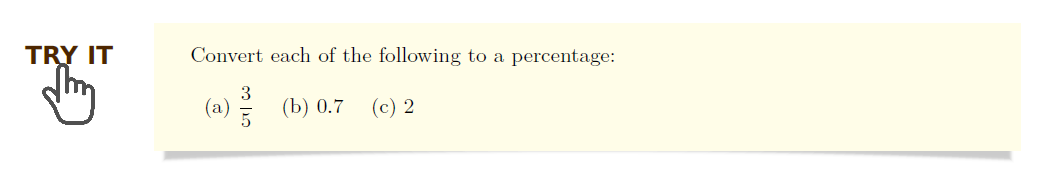
\includegraphics[width=0.75\textwidth]{tryithowto}
\end{center}

\subsection{Free Online Homework}
\parbox{0.75\textwidth}{Versatile Math includes free online homework, provided through MyOpenMath.}
\begin{center}
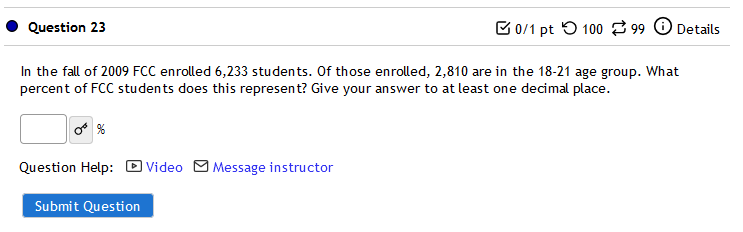
\includegraphics[width=0.75\textwidth]{homeworkscreenshot}
\end{center}
\vfill
\pagebreak

\subsection{What's New in the 2nd Edition}
\paragraph{Chapter 1}
\begin{itemize}
\item A new introduction section was added, describing many of the initial concepts used in the chapter.
\item The income tax section was moved to the end of the chapter and updated to reflect changes to the U.S. tax code (including 2020 tax brackets); the discussion of deductions and credits was expanded with new graphics.
\item The discussion of inflation was removed, since it made the section on simple and compound interest too long.
\item New examples were added to the retirement section, showing how to plan fully for retirement.
\item A description of the use of Excel and the TVM solver on TI graphing calculators was added to several sections. 
\end{itemize}

\paragraph{Chapter 2}
\begin{itemize}
\item A new section on quadratic models was added.
\item A discussion on using a calculator to do regression with each type of model was added.
\item In the section on exponential models, the discussion was condensed by eliminating models of the form $P_t = P_0e^{kt}$ and Newton's law of cooling.
\end{itemize}

\paragraph{Chapter 3}
\begin{itemize}
\item The entire chapter was reordered:
\begin{itemize}
\item The old first section was split, expanding the discussion of gathering data and graphing it into two separate sections.
\item The discussion of sampling methods was expanded, and new graphs were introduced, including dot plots and scatterplots.
\item The next two sections (measures of center and measures of spread) were merged into a single section on describing data with statistics.
\item A new section was added on the use of linear regression.
\end{itemize}
\end{itemize}

\paragraph{Chapters 4--7} These remained mostly unchanged.

\paragraph{Chapter 8} A new chapter on Graph Theory was added, with all-new videos and homework.

\paragraph{Chapter R} A short review of some algebra concepts used throughout the book was added.